\chapter{Implementación}
\label{cap:implementacion}

En éste capítulo introduciremos los detalles mas relevantes del desarrollo realizado para este trabajo. Comenzaremos mostrando la integración de nuestro sistema de NLG con \textit{Fastest}, viendo el modo de uso y los nuevos comandos introducidos para la generación de descripciones en lenguaje natural. Luego presentaremos los aspectos mas destacados de nuestra implementación para cada una de las etapas del \emph{pipeline}.

\section{Integración con \emph{Fastest}}

La implementación realizada para este trabajo se encuentra incluida en la última versión de \emph{Fastest}, cuyo código está disponible públicamente en https://github.com/rosacris/fastest. La mayor parte del código referente a este trabajo la podremos encontrar dentro del paquete \textit{main.java.nlg}.

\subsection*{Requisitos}

Deberemos cumplir con los siguientes requerimientos a fin de garantizar el correcto funcionamiento de nuestro sistema de NLG:
\begin{itemize}
 \item  \emph{Fastest 1.7 o superior \footnote{http://todo/}}: La distribución de este incluye un pequeño manual de uso.
 \item  \emph{Java SE Runtime Environment 1.6 o superior}: requerido para el correcto funcionamiento de \emph{Fastest}.
 \item  \emph{SWI\_Prolog \footnote{http://http://www.swi\_prolog.org/}}: también requerido para el correcto funcionamiento de Fastest.
 \item  \emph{FreeLing 3.1 \footnote{http://nlp.lsi.upc.edu/freeling/}\footnote{Pequeño tutorial para la instalación de \emph{FreeLing} en \emph{Ubuntu 15.04}: https://gist.github.com/juliandt/8a364d75d8b271c698aa}}: suite de análisis de lenguajes, necesaria para el módulo de NLG de \emph{Fastest}
\end{itemize}

\section{Documentación implementación}

En esta sección detallaremos los aspectos mas importantes de la implementación realizada. Para la misma respetamos la arquitectura y desarrollo realizado a lo largo de este trabajo, sin embargo podremos observar algunas diferencias menores, como por ejemplo: necesitamos modificar los nombres de las entidades intermedias utilizadas entre las distintas etapas del \textit{pipeline} para respetar las convenciones de estilo utilizadas en Fastest.

A continuación describiremos la función de los componentes mas importantes usados en cada etapa de nuestro sistema.

\subsection{\textit{Document Planner}}

El módulo \emph{DocumentPlanner} será el encargado de llevar a cabo las tareas de determinación de contenido y estructuración del documento detalladas en el capítulo \ref{cap:document_planning}. En la figura \ref{fig:imp_documentplanner} podemos observar los componentes mas importantes involucrados en esta etapa, cuya función describiremos a continuación. 

\begin{figure}[H]
  	\centering
	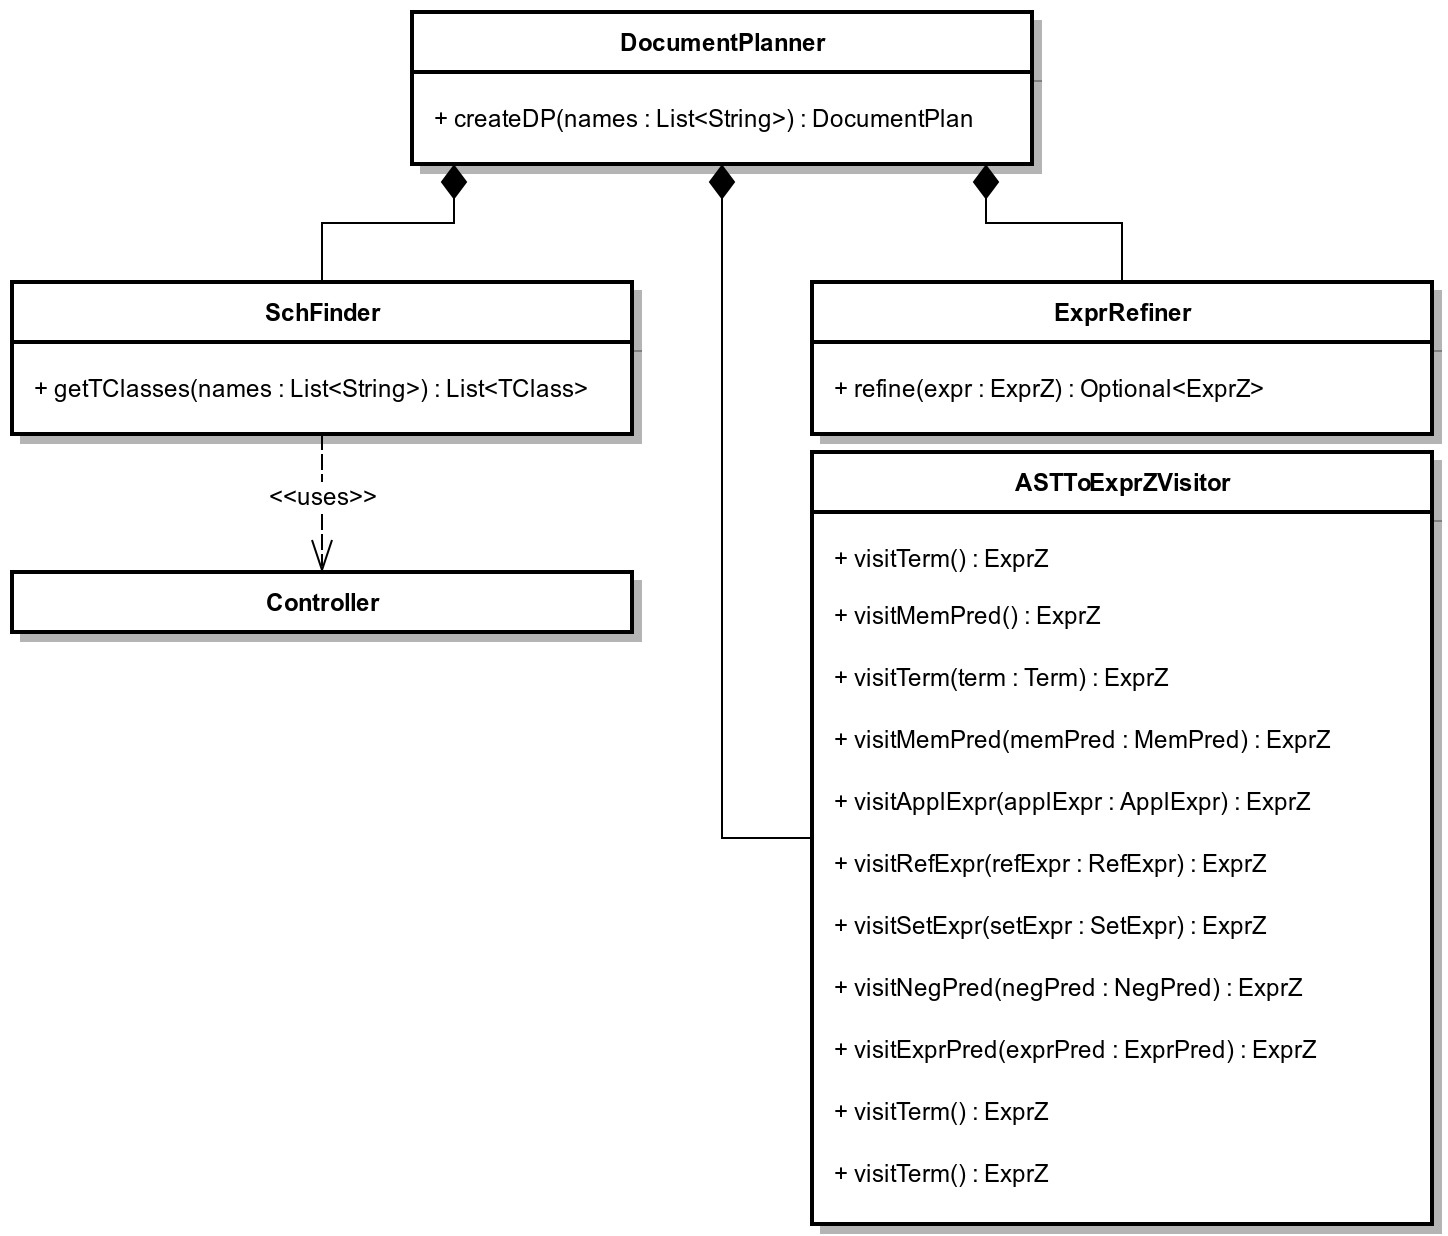
\includegraphics[scale=0.25]{img/documentplanner_imp.png}
	\caption{Diagrama clases \textit{DocumentPlanner}}
  	\label{fig:imp_documentplanner}
\end{figure}

\bigskip
\noindent
\textbf{DocumentPlanner.} Es el módulo encargado de crear un \textit{document plan} a partir de la entrada de nuestro sistema. Construye los mensajes y estructuras intermedias de éste delegando las tareas de determinación de contenido en los módulos que describiremos a continuación.

\bigskip
\noindent
\textbf{SchFinder.} La tarea de selección detallada en el capítulo \ref{cap:determinacion_contenido} será desarrollada por este módulo. Este será el encargado de recuperar el conjunto de clases de prueba indicadas. El mismo posee una referencia al \emph{Controller} \footnote{Es el módulo encargado de mantener las referencias a elementos de la especificación, arboles de prueba, etc.} de Fastest que le permitirá identificar y recuperar las clases de prueba necesarias. 


\bigskip
\noindent
\textbf{ExprRefiner.} Es la \textit{fachada} \cite{gof} encargada de delegar los distintos procesamientos a realizar sobre las expresiones a fin de desarrollar las tareas de eliminación de tautologías y reducción de expresiones estudiadas también en el capítulo \ref{cap:determinacion_contenido}. Podemos observar que utilizamos la clase \emph{Optimal} de Java 8 para modelar el hecho de que el método \textbf{refine()} podría no devolver un valor, por ejemplo en el caso que la expresión procesada sea una tautología y no deba ser incluida en el \textit{document plan}.

\bigskip
Fastest utiliza el \textit{framework} CZT \footnote{http://czt.sourceforge.net/} que integra un conjunto de herramientas para trabajar con el lenguaje de especificación Z. La forma en la que CZT modela las expresiones de Z nos resultó demasiado compleja para este trabajo, por lo que decidimos transformar las expresiones contempladas dentro del alcance de este trabajo a un modelo más simple (los que nos simplificará posteriormente la implementación del algoritmo de lexicalización, por ejemplo). En la figura \ref{fig:imp_exprz} podemos observar la jerarquía de clases de las expresiones utilizadas en este trabajo para modelar las expresiones Z. 

\begin{figure}[H]
  	\centering
	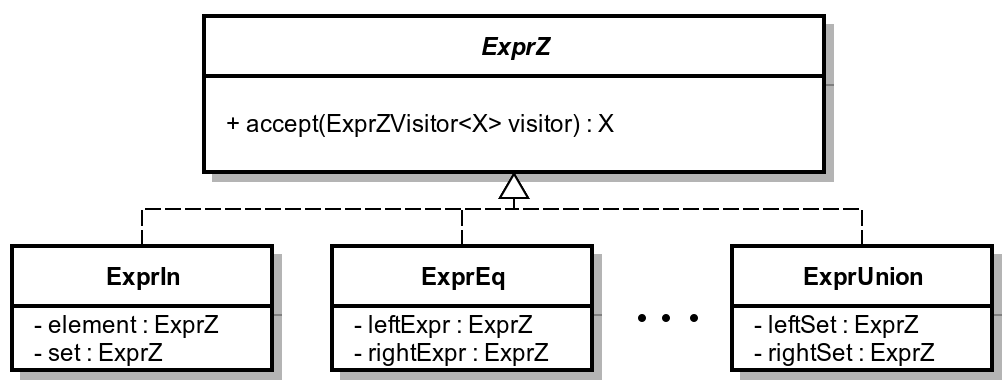
\includegraphics[scale=0.31]{img/exprz_imp.png}
	\caption{Diagrama jerarquía de clases ExprZ}
  	\label{fig:imp_exprz}
\end{figure}

\bigskip
\noindent
\textbf{ASTToExprZVisitor.} Este módulo será el responsable de la transformación entre el modelo de CZT y el utilizado por este trabajo presentado anteriormente.


\subsection{\textit{Microplanner}}

En esta sección presentaremos los componentes encargados de la tarea de \textit{microplanning} detallada en el capítulo \ref{cap:microplanning}. En la figura \ref{fig:imp_microplanner} podemos observar los módulos involucrados en la implementación de esta tarea.

\begin{figure}[H]
  	\centering
	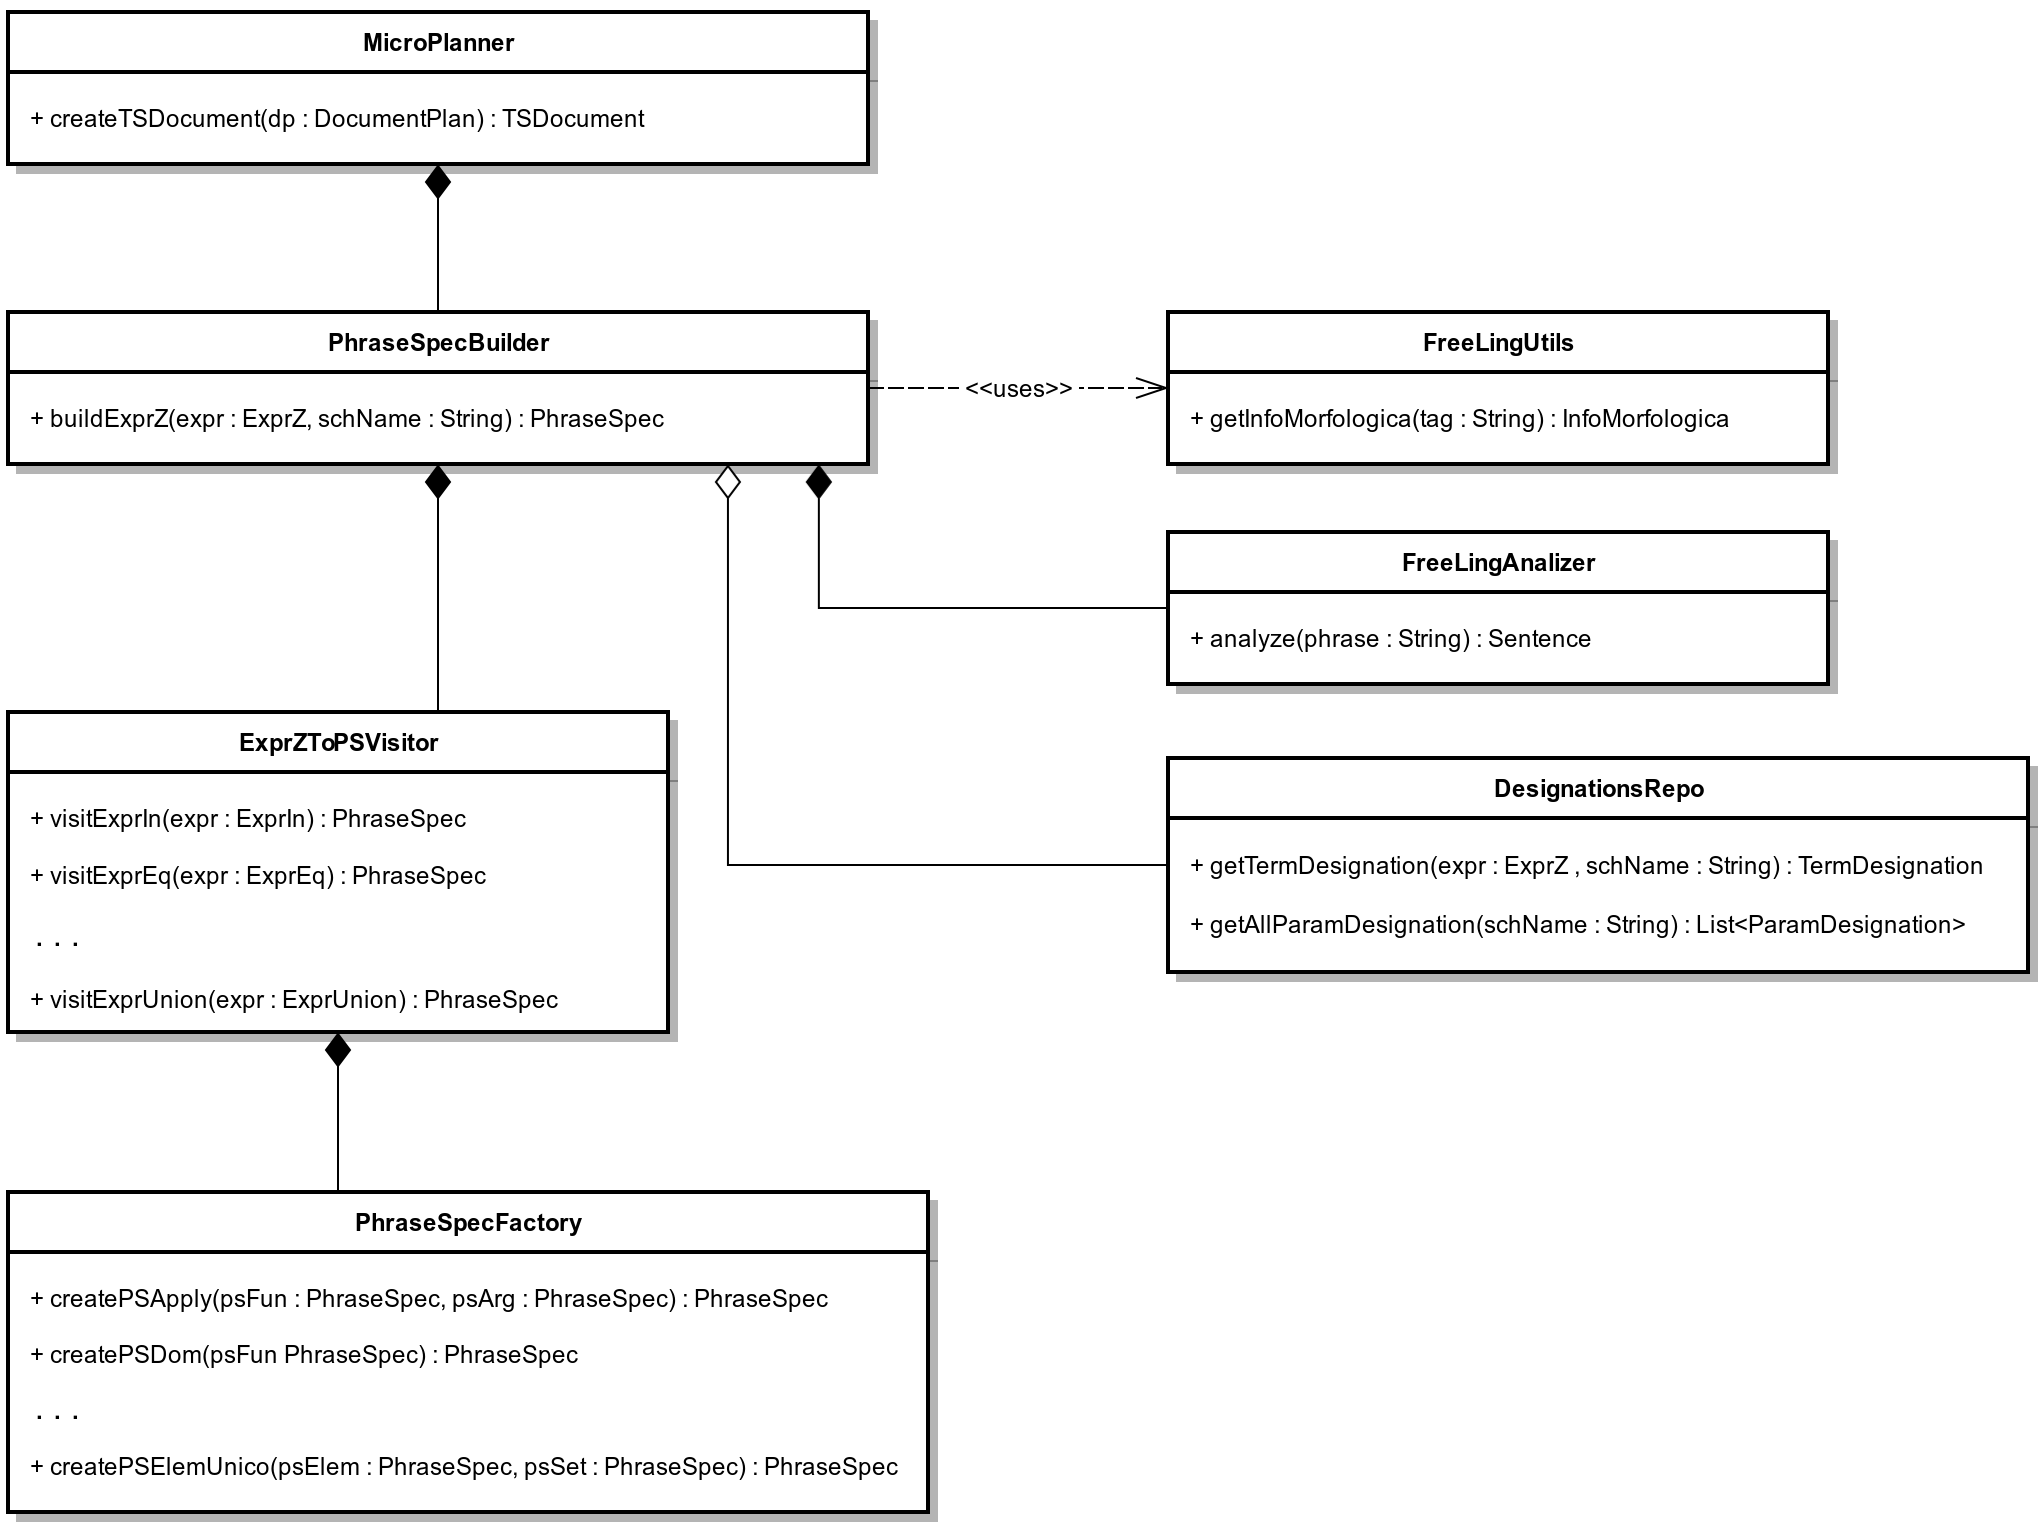
\includegraphics[scale=0.2]{img/microplanner_imp.png}
	\caption{Diagrama clases \textit{Microplanner}}
  	\label{fig:imp_microplanner}
\end{figure}

\bigskip
\noindent
\textbf{MicroPlanner.} Es el módulo encargado de construir la especificación del documento a partir del \textit{document plan} generado por la etapa anterior, delegando la tarea de lexicalización en \textbf{PhraseSpecBuilder}.

\bigskip
\noindent
\textbf{PhraseBuilder.} Este módulo implementa la tarea de lexicalización detallada en el capítulo \ref{cap:microplanning}. Este tiene la tarea de construir una especificación de frase a partir de una expresión Z. Delegamos en el módulo \textbf{ExprZToPSVisitor} el análisis de casos para las distintas expresiones y sus posibles combinaciones.

\bigskip
\noindent
\textbf{ExprZToPSVisitor.} Encapsula las reglas de lexicalización para todas las posibles expresiones y combinaciones de las mismas. Implementa la función auxiliar \textit{lexicalización'()} utilizada en el bosquejo de la figura \ref{fig:algoritmo_lexicalizacion}.

\bigskip
\noindent
\textbf{PhraseSpecFactory.} Módulo encargado de construir apropiadamente las distintas especificaciones de frase de nuestro sistema. Por ejemplo: \textit{createPSElemUnico()} compondrá dos especificaciones de frase para generar la especificación de la frase \textit{``... es el único elemento de ...''} siendo las dos especificaciones mencionadas anteriormente las encargadas de modelar el texto que precede y antecede respectivamente al anterior.

\bigskip
\noindent
\textbf{FreeLingAnalizer.} Como ya mencionamos previamente, utilizamos el analizador FreeLing para obtener las características morfológicas de los distintos constituyentes de las frases utilizadas en las designaciones. Este módulo tendrá la tarea de interactuar con FreeLing proveyéndonos de la información necesaria (como cual es el núcleo de la frase, cual es su genero, número, etc.) para construir una especificación de frase a partir de una designación.

\bigskip
\noindent
\textbf{FreeLingUtils.} Contiene algunas métodos útiles para el trabajo con FreeLing. Por ejemplo, FreeLing genera una estructura en la que etiqueta cada palabra con anotaciones morfosintácticas, el método \textit{morfosintáctica()} procesa estas anotaciones produciendo una estructura mas sencilla con la que trabajará nuestro sistema.

\bigskip
\noindent
\textbf{DesignationsRepo.} Es necesario para el algoritmo de lexicalización saber si una expresión se encuentra designada y cual es su designación en el caso de estarlo. Será a través de este módulo que podrá acceder a las designaciones presentes en la especificación. El mismo se inicializa al cargar la especificación en Fastest. 

%TODO cambiar nombres a español
\subsection{\textit{Surface Realizer}}

\begin{figure}[H]
  	\centering
	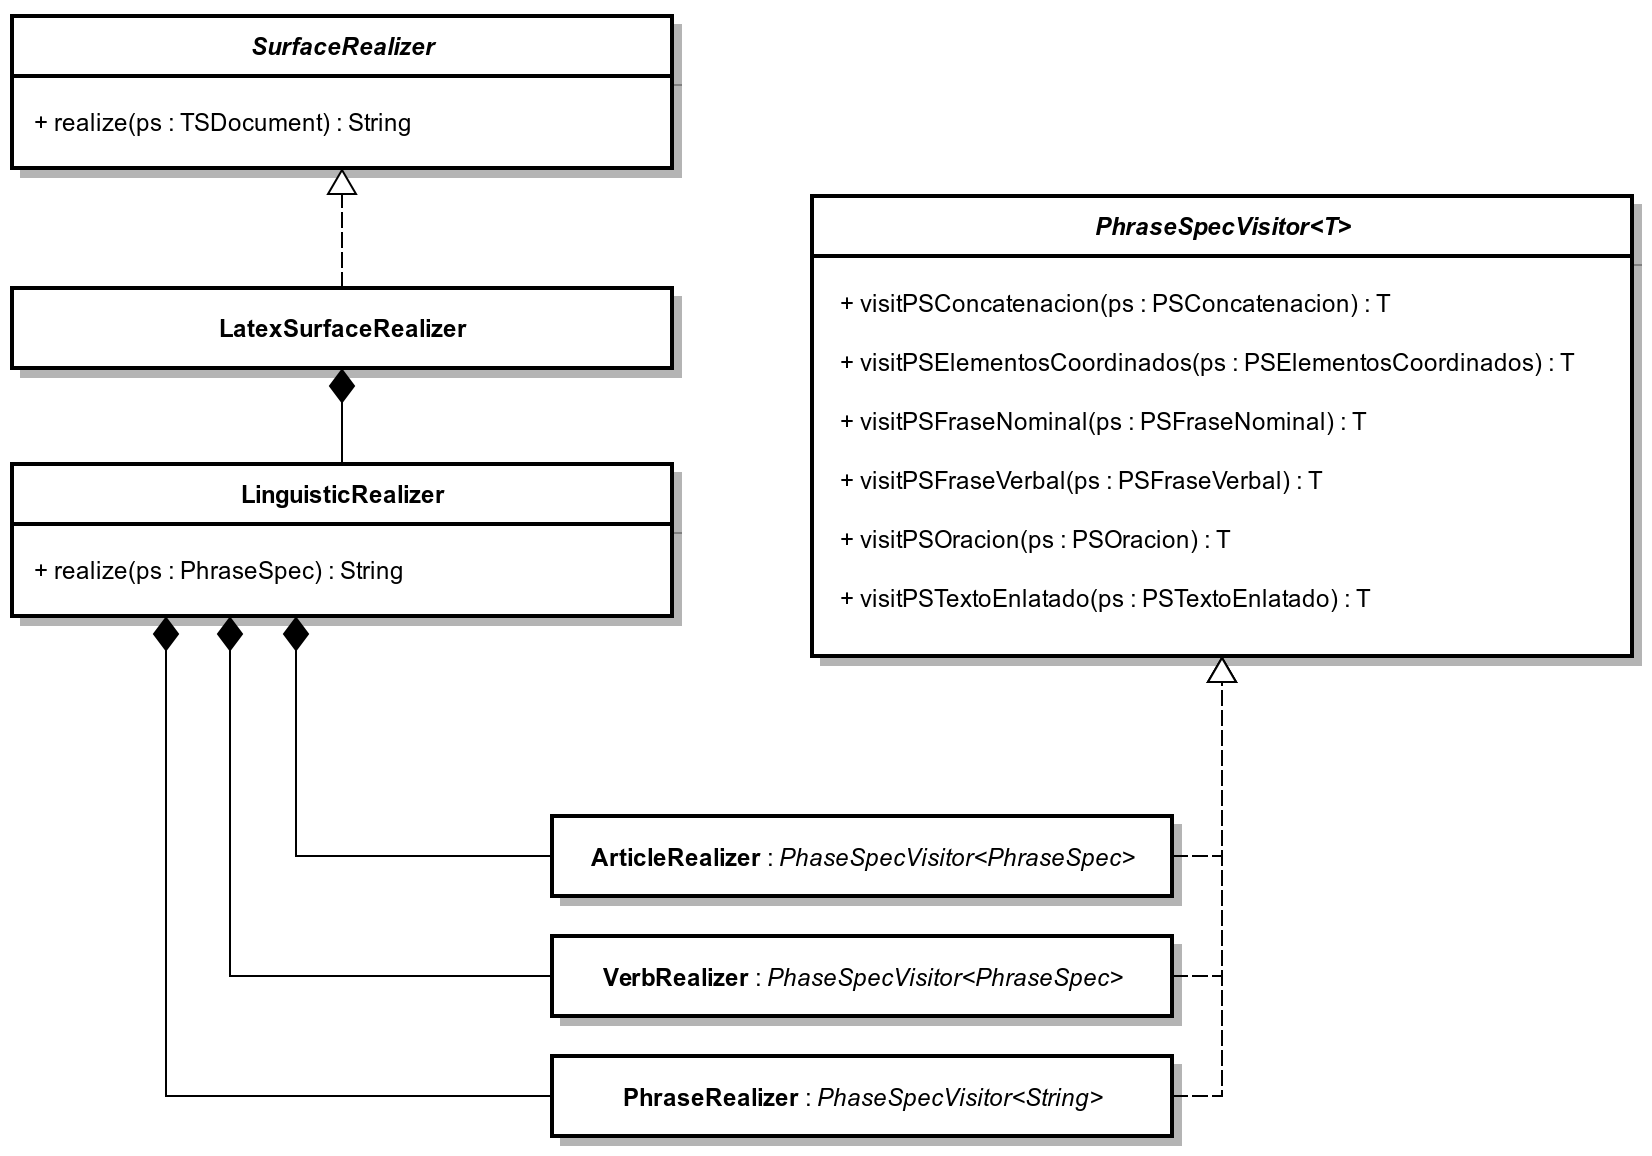
\includegraphics[scale=0.17]{img/realizer_imp.png}
	\caption{Diagrama clases \textit{Surface Realizer}}
  	\label{fig:imp_surfrealizer}
\end{figure}

\bigskip
\noindent
\textbf{SurfaceRealizer.} Lorem ipsum dolor sit amet, consectetur adipiscing elit, sed do eiusmod tempor incididunt ut labore et dolore magna aliqua. Ut enim ad minim veniam, quis nostrud exercitation ullamco laboris nisi ut aliquip ex ea commodo consequat.

\bigskip
\noindent
\textbf{LinguisticRealizer.} Lorem ipsum dolor sit amet, consectetur adipiscing elit, sed do eiusmod tempor incididunt ut labore et dolore magna aliqua. Ut enim ad minim veniam, quis nostrud exercitation ullamco laboris nisi ut aliquip ex ea commodo consequat.

\bigskip
\noindent
\textbf{PhraseSpecVisitor.} Lorem ipsum dolor sit amet, consectetur adipiscing elit, sed do eiusmod tempor incididunt ut labore et dolore magna aliqua. Ut enim ad minim veniam, quis nostrud exercitation ullamco laboris nisi ut aliquip ex ea commodo consequat.

\bigskip
\noindent
\textbf{ArticleRealizer.} Lorem ipsum dolor sit amet, consectetur adipiscing elit, sed do eiusmod tempor incididunt ut labore et dolore magna aliqua. Ut enim ad minim veniam, quis nostrud exercitation ullamco laboris nisi ut aliquip ex ea commodo consequat.

\bigskip
\noindent
\textbf{VerbRealizer.} Lorem ipsum dolor sit amet, consectetur adipiscing elit, sed do eiusmod tempor incididunt ut labore et dolore magna aliqua. Ut enim ad minim veniam, quis nostrud exercitation ullamco laboris nisi ut aliquip ex ea commodo consequat.

\bigskip
\noindent
\textbf{PhraseRealizer.} Lorem ipsum dolor sit amet, consectetur adipiscing elit, sed do eiusmod tempor incididunt ut labore et dolore magna aliqua. Ut enim ad minim veniam, quis nostrud exercitation ullamco laboris nisi ut aliquip ex ea commodo consequat.